\def \imgpath {"./figures/alice"}

The experimental measurements conducted as part of this dissertation in Chapters~\ref{chap:sphero} and \ref{chap:rt} have been carried out on data from proton-proton collisions at the Large Hadron Collider at CERN, collected with the ALICE detector. The aim of this chapter is to introduce these facilities.

\section{CERN and the LHC}

\textit{Conseil européen pour la recherche nucléaire} (CERN) is a scientific institution dedicated to study particle physics, nuclear physics, and related fields. It was established in 1954 as a European collaborative endeavour and currently has 23 member states. The CERN laboratories employ almost 3000 on-site staff and host approx.\ 13000 users from universities and research institutions across the world. The biggest achievments of CERN include discoveries of the $W^\pm$, $Z^0$, \cite{cashmorePrestigiousDiscoveriesCERN2003} and the Higgs bosons \cite{thecmscollaborationObservationNewBoson2012, theatlascollaborationObservationNewParticle2012}, the first creation of anti-atoms, advancements to proton therapy and medical imaging technologies such as PET, and finally, being a birthplace to the World Wide Web.

The Large Hadron Collider (LHC) is the main particle accelerator at CERN. This synchrotron with circumference of almost 27 km can accelerate protons to energies up to $7$~TeV, making it world's most powerful particle accelerators. Apart from collisions of protons measured at \sppt{13}, it also studies collisions of nuclei, such as lead (Pb-Pb) at \snnt{5.02}, or proton-lead p-Pb at \snnt{8.16}. Particles in the synchrotron are accelerated by electric fields within RF cavities and kept on their semi-circular trajectory using magnetic dipoles. Higher-polar magnets are used for beam focusing and adjustment. The particles circulate in larger bunches (of $\sim 10^{11}$ protons or $\sim 7\times10^7$ Pb nuclei) in two separate rings, which intersect at sites of large experiments, detecting their collisions. Apart from ALICE, discussed in the next sections, these are:
\begin{itemize}
\item \textbf{ATLAS} (\textit{A Toroidal LHC ApparatuS}) \cite{collaborationATLASExperimentCERN2008}: the LHC's largest experiment and a general purpose detector, with its foci including Higgs physics, scrutiny of the SM, and BSM searches.
\item \textbf{CMS} (\textit{Compact Muon Solenoid}) \cite{collaborationCMSExperimentCERN2008}: also a general purpose detector, with similar physics goals, but with a different technical design than ATLAS. It has also been a prominent contributor to QGP physics, particularly the study of small systems.
\item \textbf{LHCb} (\textit{Large Hadron Collider beauty}) \cite{collaborationLHCbDetectorLHC2008}: a detector focused mostly on precise measurements of b physics and CP violation. 
\end{itemize}

\begin{table}[h!]
\centering
\caption{Selection of parameters of the Large Hadron Colliders. \cite{schmidtProtectionCERNLarge2006} }
\label{tab:alice:lhcpars}
\begin{tabular}{|cc|c|}
\hline
\multicolumn{2}{|c|}{\parbox[b][1.2em]{2em}{} Parameter} & Value \\ \hline
\multicolumn{2}{|l|}{\parbox[b][1.1em]{1em}{}Circumference} &  $26.7$ km\\ \hline
\multicolumn{2}{|l|}{\parbox[b][1.1em]{1em}{}Energy at injection} &  $450$ GeV\\ \hline
\multicolumn{2}{|l|}{\parbox[b][1.1em]{1em}{}Magnetic field at 7 TeV} &  $\sim 8.3$ T\\ \hline
\multicolumn{2}{|l|}{\parbox[b][1.1em]{1em}{}Number of magnets} &  $\sim 9300$\\ \hline
\multicolumn{2}{|l|}{\parbox[b][1.1em]{1em}{}Revolution frequency} &  $\sim 11$ kHz\\ \hline
\multicolumn{2}{|l|}{\parbox[b][1.1em]{1em}{}Number of bunches in a beam} &  $2808$\\ \hline
\multicolumn{2}{|l|}{\parbox[b][1.1em]{1em}{}Bunch spacing} &  $25$ ns\\ \hline
\multicolumn{2}{|l|}{\parbox[b][1.1em]{1em}{}Design luminosity} &  $\sim 10^{34} \, \mathrm{cm^{-2}s^{-1}}$\\ \hline
\multicolumn{2}{|l|}{\parbox[b][1.1em]{1em}{}Max.\ bunch crossing (BC) rate} &  $\sim 40$ MHz\\ \hline
\multicolumn{2}{|l|}{\parbox[b][1.1em]{1em}{}Number of inel.\ interactions per BC} &  $10-20$\\ \hline
\multicolumn{2}{|l|}{\parbox[b][1.1em]{1em}{}Beam lifetime} &  $\sim 10$ h\\ \hline
\end{tabular}
\end{table}

Some of the LHC parameters are summarised in Tab.~\ref{tab:alice:lhcpars} and an aerial photo of the LHC with locations of the IPs can be seen in Fig.~\ref{fig:alice:lhc}.

\begin{figure}%[!h]
\subfloat[][]{\adjincludegraphics[trim={0 {.18\height} 0 {.07\height}},clip,width=.8\textwidth]{\imgpath/lhc.jpg}}\\
\subfloat[][]{\adjincludegraphics[trim={0 {.08\height} 0 {.07\height}},clip,width=.8\textwidth]{\imgpath/ip.jpg}}
\caption{\textbf{(a)} Aerial photo of the LHC area, also depicting the location of the LHC tunnel (approx.\ $100$~m underground), spanning over Switzerland and France. Geneva, Lac Léman, and the Mont Blanc can be seen in the background. \cite{briceAerialViewCERN2008} \textbf{(b)} Visualisation of the beam crossing at the ALICE experiment. Bunches of Beam 1 move from left to right in the blue beam envelope and bunches of Beam 2 move from right to left in the red beam envelope. The envelopes indicate the beam orbits and transverse size. \cite{LHCReportMake2023}}
\label{fig:alice:lhc}
\end{figure}

\section{The ALICE experiment}

The ALICE (A Large Ion Collider Experiment) \cite{collaborationALICEExperimentCERN2008, PerformanceALICEExperiment2014} is the detector at the LHC dedicated to studying collisions of heavy nuclei and the properties of QCD matter, such as quark-gluon plasma. Its biggest strengths are precise tracking and momentum determination all the way down to $\pt>\gevc{0.15}$ as well as superior particle identification (PID). Its sub-detectors are subjected to a magnetic field of $0.5$~T to allow momentum measurements from the track curvatures (in natural units, $\pt \approx 0.3 B r, \, \pt \in [\gevc{}], \, B \in [\mathrm{T}], \, r \in [\mathrm{m}]$).

The ALICE detector, shown in Fig.~\ref{fig:alice:alice}, consists of several sub-systems, each fulfilling their function. Some of them which pertain to the measurements carried out within this dissertation are listed in Tab.~\ref{tab:alice:alice}. The following descriptions are based on their status when the data was collected, which corresponds to Run~2.

\begin{figure}[H]
\centering%
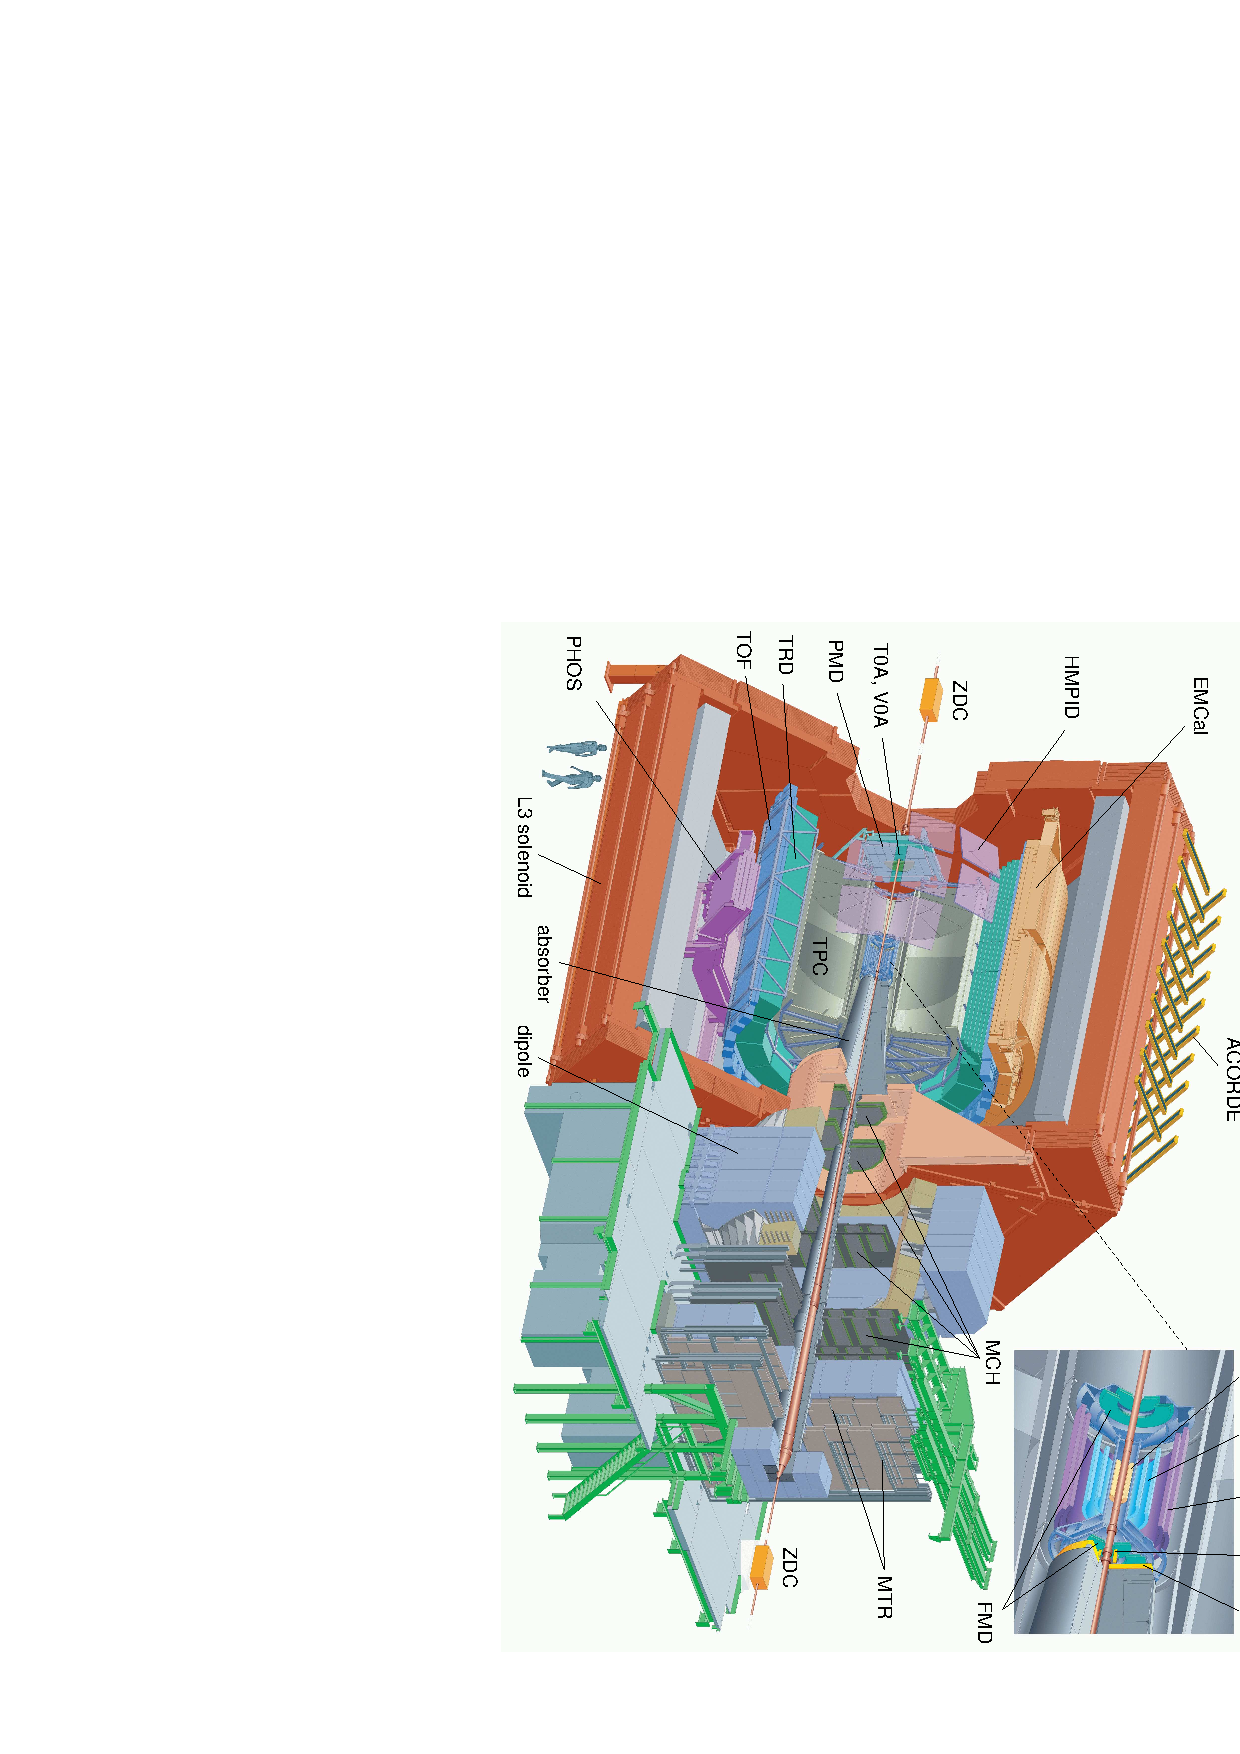
\includegraphics[width=.99\textwidth]{\imgpath/setup7.pdf}
\caption{The ALICE experiment at the LHC, showing its sub-systems. The central barrel is subjected to a magnetic field from the solenoid (red). The ZDC detectors are approximately $\pm 113$~m distant from the IP. \cite{alicecollaborationPerformanceALICEExperiment2014}}
\label{fig:alice:alice}
\end{figure}

\begin{table}[h!]
\centering
\caption{Selection of ALICE sub-detectors relevant to this thesis. Acceptance is given in terms of pseudorapidity, the azimuthal coverage for the detectors presented is full. The $z$-axis is defined anticlockwise to the LHC. \cite{alicecollaborationPerformanceALICEExperiment2014} }
\label{tab:alice:alice}
\begin{tabular}{|cc|cccc|}
\hline
\multicolumn{2}{|c|}{\parbox[b][1.2em]{2em}{} Detector} & Acceptance & Position (cm) & Technology & Main purpose \\ \hline
\multicolumn{6}{l}{\parbox[b][0.2em]{1em}{}} \\
\hline
\multicolumn{2}{|c|}{\parbox[b][1.2em]{2em}{} ITS SPD} & $|\eta|<2.0$ & $r=3.9$ cm & Si pixel & tracking, PV, triggering \\
\multicolumn{2}{|c|}{\parbox[b][1.2em]{2em}{} ITS SPD} & $|\eta|<1.4$ & $r=7.6$ cm & Si pixel & tracking, PV, triggering \\
\hline
\multicolumn{2}{|c|}{\parbox[b][1.2em]{2em}{} ITS SDD} & $|\eta|<0.9$ & $r=15.0$ cm & Si drift & tracking, PID \\
\multicolumn{2}{|c|}{\parbox[b][1.2em]{2em}{} ITS SDD} & $|\eta|<0.9$ & $r=23.9$ cm & Si drift & tracking, PID \\
\hline
\multicolumn{2}{|c|}{\parbox[b][1.2em]{2em}{} ITS SSD} & $|\eta|<1.0$ & $r=38.0$ cm & Si strip & tracking, PID \\
\multicolumn{2}{|c|}{\parbox[b][1.2em]{2em}{} ITS SSD} & $|\eta|<1.0$ & $r=43.0$ cm & Si strip & tracking, PID \\
\hline
\multicolumn{2}{|c|}{\parbox[b][1.2em]{2em}{} TPC} & $|\eta|<0.9$ & $r=85.0$ cm & Ne drift, MWPC & tracking, PV, PID \\
\hline
\multicolumn{2}{|c|}{\parbox[b][1.2em]{2em}{} \VOA} & $2.8<|\eta|<5.1$ & $z=329.0$ cm & scintillator & centrality, triggering \\
\multicolumn{2}{|c|}{\parbox[b][1.2em]{2em}{} \VOC} & $-3.7<|\eta|<-1.7$ & $z=-88.0$ cm & scintillator & centrality, triggering \\
\hline
\end{tabular}
\end{table}


\section{Time Projection Chamber}

The Time Projection Chamber (TPC) \cite{peskovTechnicalDesignReport2014} is ALICE's primary tracking detector and investigation tool for hadronic observables. It is located in the central barrel. The cylinder, illustrated in Fig.~\ref{fig:alice:tpc} is filled with a mixture of gases and a central $100$-kV high-voltage electrode subjects it to a longitudinal electric field. Charged particles traversing the gas medium ionise it and the electrons then drift to the end-caps with a drift time of approx.\ $90 \, \mathrm{\mu s}$. There, they are detected in Read-out Chambers (ROCs), using Multi-Wire Proportional Chambers (MWPC), and together with the drift duration time, a three-dimensional information can be determined. The ROCs are radially divided (IROCs and OROCs) and segmented into 18 sectors in azimuth. Each ROC has 159 rows and its signals are processed by attached Front-End Cards (FECs). The MWPC principle and the ROC design, visualised with a charged particle track crossing all its rows, can be seen in Fig.~\ref{fig:alice:rocs}.

In addition to the tracking information, the TPC is also used in PID, by measuring the charged particles' specific ionisation loss $\mathrm{d}E/\mathrm{d}x$. Measurements of $\mathrm{d}E/\mathrm{d}x$ for different particle species as a function of the particle momentum and charge is displayed in Fig.~\ref{fig:alice:tpc}. A selection of TPC parameters not discussed above is given in Tab.~\ref{tab:alice:tpc}.

\begin{table}[h!]
\centering
\caption{Selection of parameters of the Time Projection Chamber. \cite{collaborationALICEExperimentCERN2008} }
\label{tab:alice:alice}
\begin{tabular}{|cc|c|}
\hline
\multicolumn{2}{|c|}{\parbox[b][1.2em]{2em}{} Parameter} & Value \\ \hline
\multicolumn{2}{|l|}{\parbox[b][1.1em]{1em}{}Radial position (active volume)} &  $84.8<r<246.6$ cm\\ \hline
\multicolumn{2}{|l|}{\parbox[b][1.1em]{1em}{}Length (active volume)} &  $2\times250$ cm\\ \hline
\multicolumn{2}{|l|}{\parbox[b][1.1em]{1em}{}Detector gas} &  Ne/CO$_2$/N$_2$ or Ar/CO$_2$\\ \hline
\multicolumn{2}{|l|}{\parbox[b][1.1em]{1em}{}Spatial resolution} &  $0.8-1.1$ mm in $r\phi$\\
\multicolumn{2}{|l|}{\parbox[b][1.1em]{1em}{} } &  $1.1-1.2$ mm in $z$\\ \hline
\multicolumn{2}{|l|}{\parbox[b][1.1em]{1em}{}$\mathrm{d}E/\mathrm{d}x$ resolution} &  $\sim 5.0\%$\\ \hline
\multicolumn{2}{|l|}{\parbox[b][1.1em]{1em}{}Material budget $X/X_0$} &  $3.5\%$ near $\eta=0$\\ \hline
\end{tabular}
\end{table}

\begin{figure}[!h]
\subfloat[][]{\adjustbox{valign=m}{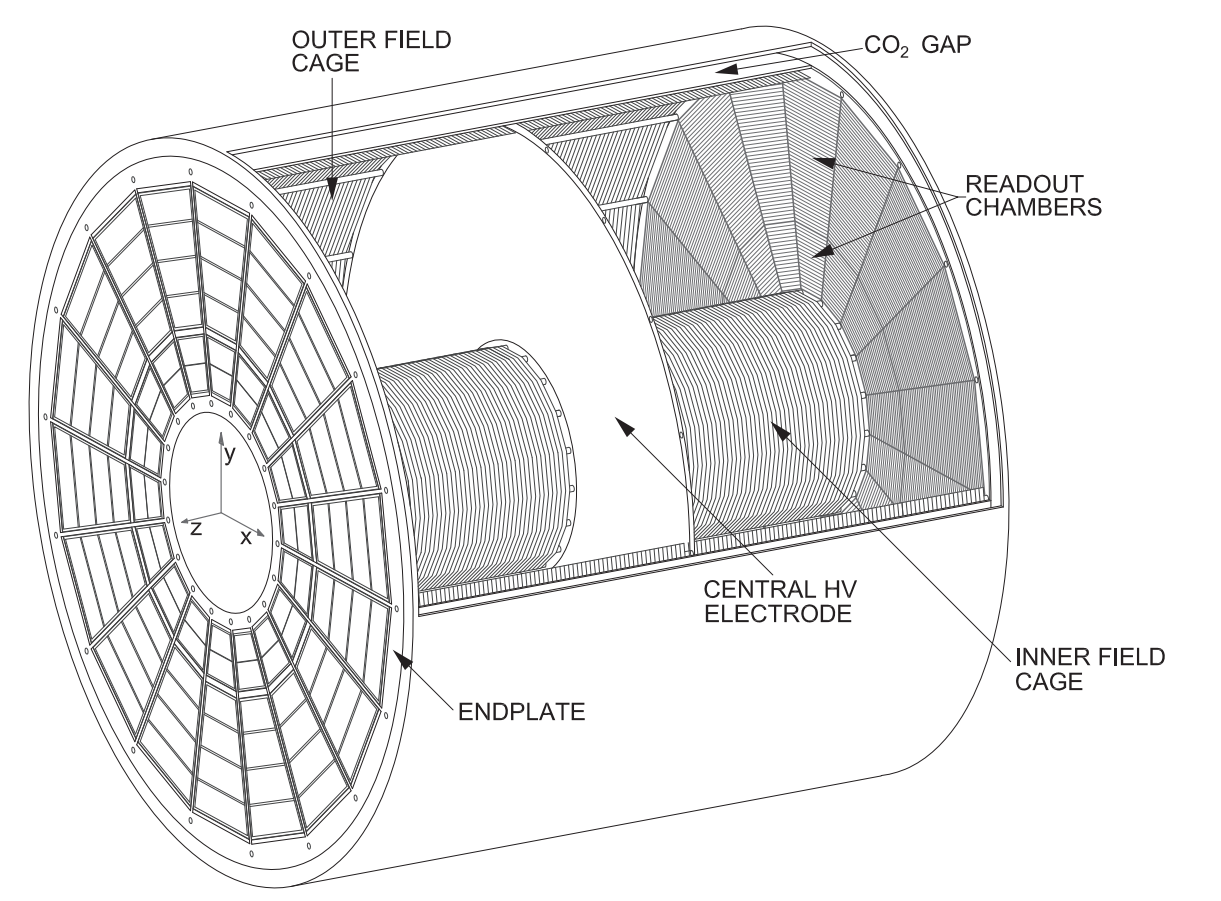
\includegraphics[width=.47\textwidth]{\imgpath/tpc.png}}}
\subfloat[][]{\adjustbox{valign=m}{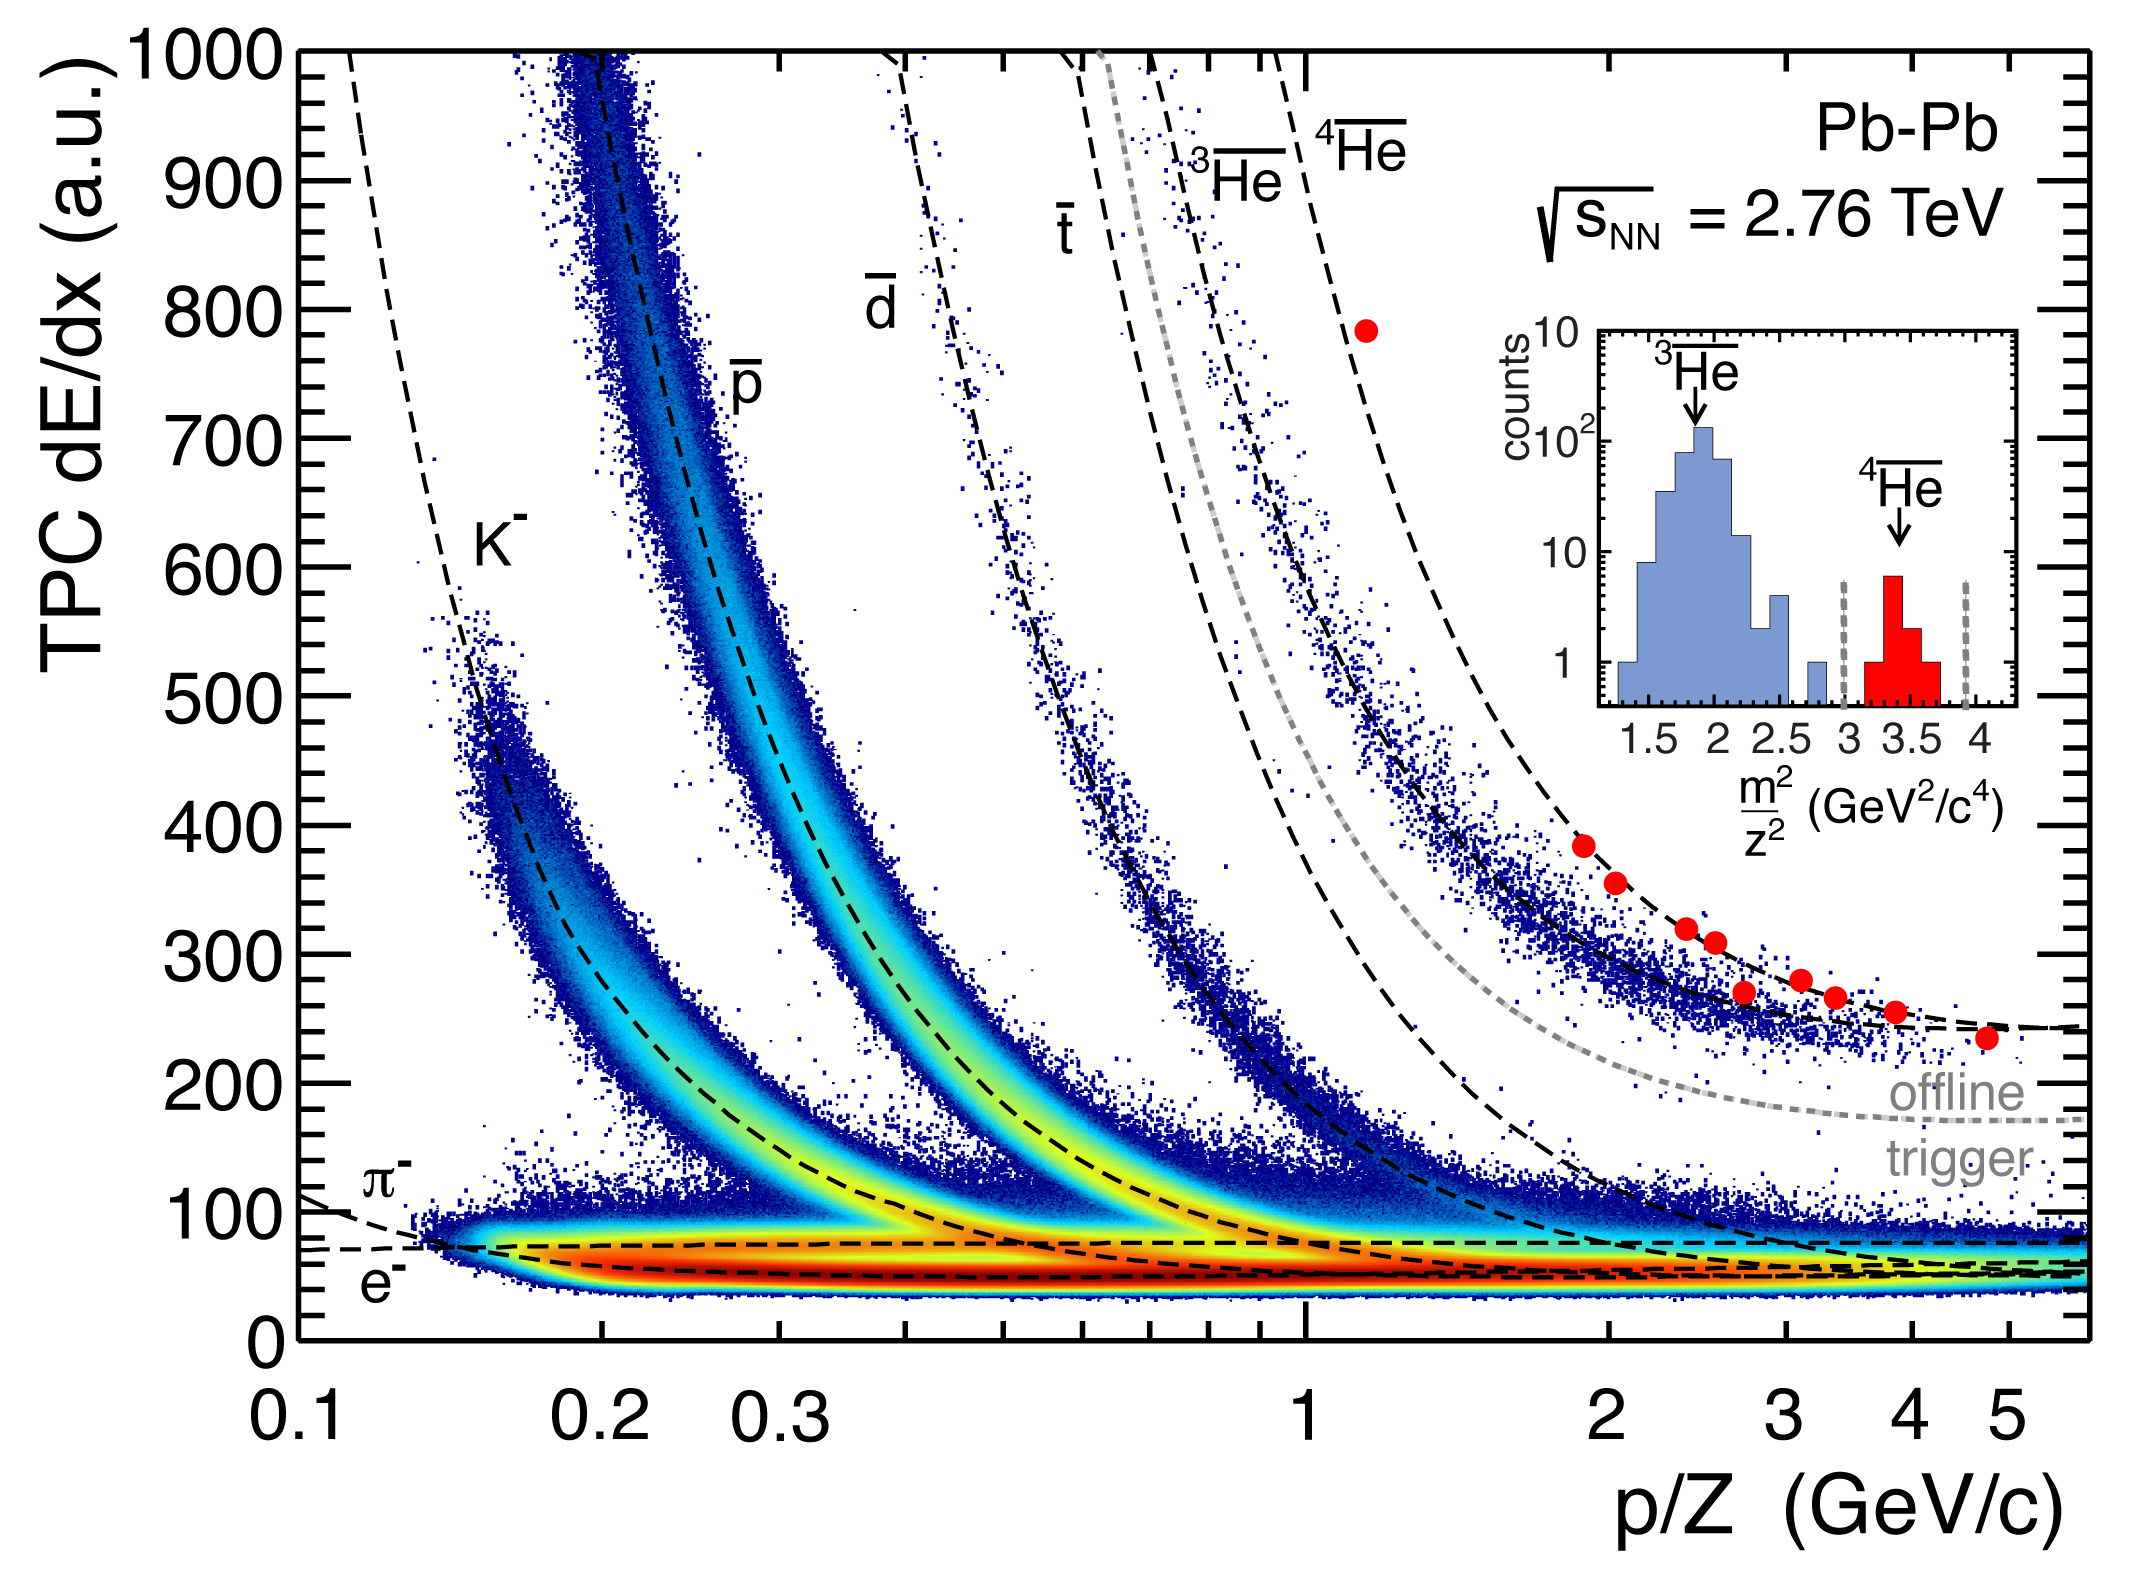
\includegraphics[width=.47\textwidth]{\imgpath/dedx.eps}}}
\caption{\textbf{(a)} Illustration of the TPC detector. \cite{peskovTechnicalDesignReport2014}. \textbf{(b)} Ionisation energy loss of charged particles as a function of their momentum normalised by their charge as determined by the TPC. The dashed lines represent predictions from calculations. \cite{alicecollaborationPerformanceALICEExperiment2014}}
\label{fig:alice:tpc}
\end{figure}

\begin{figure}[!h]
\subfloat[][]{\adjustbox{valign=m}{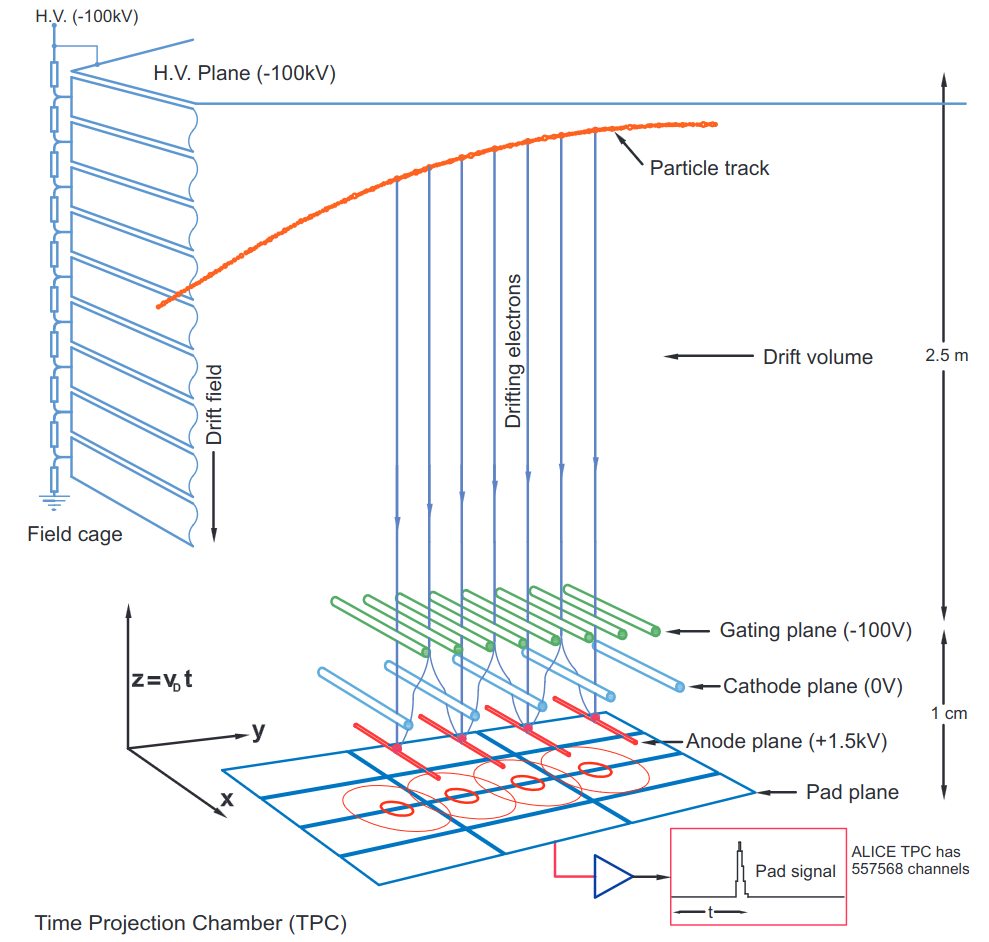
\includegraphics[width=.45\textwidth]{\imgpath/mwpc.png}}}
\subfloat[][]{\adjustbox{valign=m}{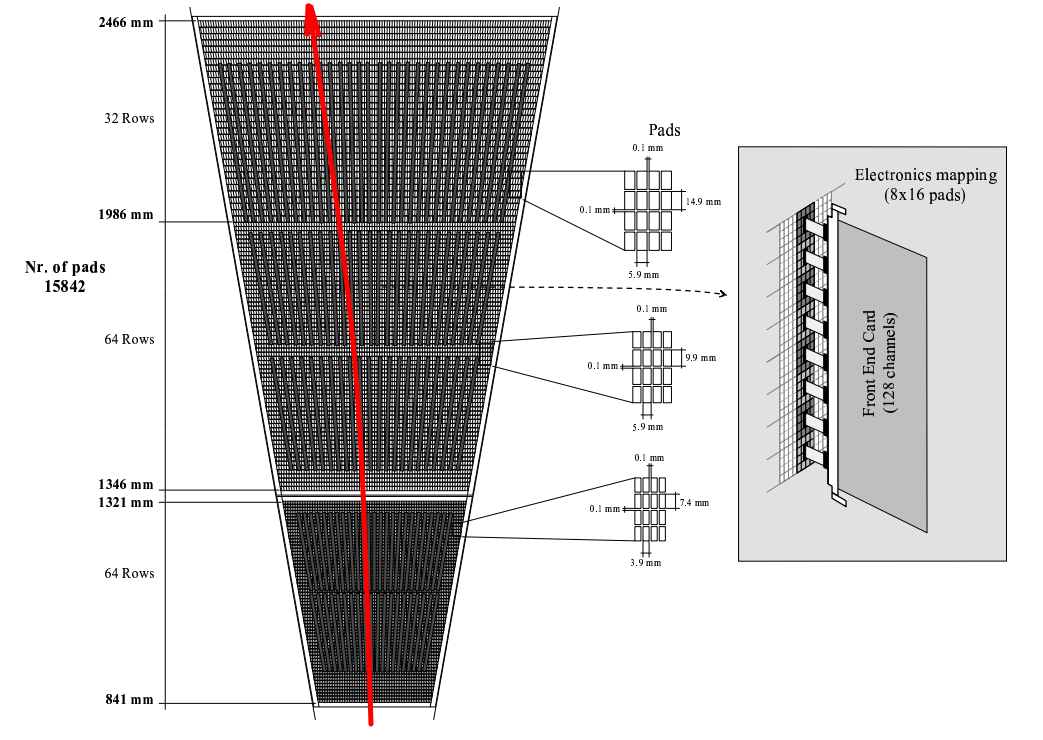
\includegraphics[width=.45\textwidth]{\imgpath/fec2.png}}}
\caption{\textbf{(a)} Depiction of the operating principle at the ROCs, using MWPC. \cite{kalweitProductionLightFlavor2012} \textbf{(b)} The IROC (bottom part) and OROC (top part) visualised with their number of rows and the signal-processing FECs. Also shown is a charged particle trajectory (red), which in this case crosses all 159~rows. \cite{peskovTechnicalDesignReport2014} (\textit{modified})}
\label{fig:alice:rocs}
\end{figure}


\subsection{Upgrade for Run 3: GEM read-outs}

In the Run 2 setup, to avoid build-up of space charge in the TPC due to backflow of ions from the amplification region in MWPCs, a gating grid is used. This limits the operating rate of the TPC to approx.\ $3.5$~kHz. However, for the Run 3 operation, the TPC has been planned to enable a continous read-out mode of Pb-Pb collisions at the interaction rate $50$~kHz. For this reason, a new read-out technology, the Gas Electron Multiplier (GEM), is used. The technology and upgraded are discussed in more detail in Ref.~\cite{adolfssonUpgradeALICETPC2021}. Commissioning of this upgraded TPC comprised the author's qualification task.

The GEM uses $50$-$\mathrm{\mu m}$ thin foils of insulating material, coated with conductive layers of thickness $2-5$ $\mathrm{\mu m}$ at each side, to which a potential difference of $200-400$~V is applied. The foil is perforated with double-conical holes of diameters $\sim 70$ and $\sim 50$ $\mathrm{\mu m}$ and a pitch of $\sim 140$ or $\sim 280$~$\mathrm{\mu m}$. The electric field in the holes than causes avalanche multiplication. Four GEM layers are stacked on top of each other in a way, where the holes have different positions and densities, which reduces the ion backflow. Typically, for one electron, the gain is around $2000$, with $20$ ions flowing back into the drifting region. The GEM setup at ALICE is displayed in Fig.~\ref{fig:alice:gems}.

\begin{figure}[!h]
\subfloat[][]{\adjustbox{valign=m}{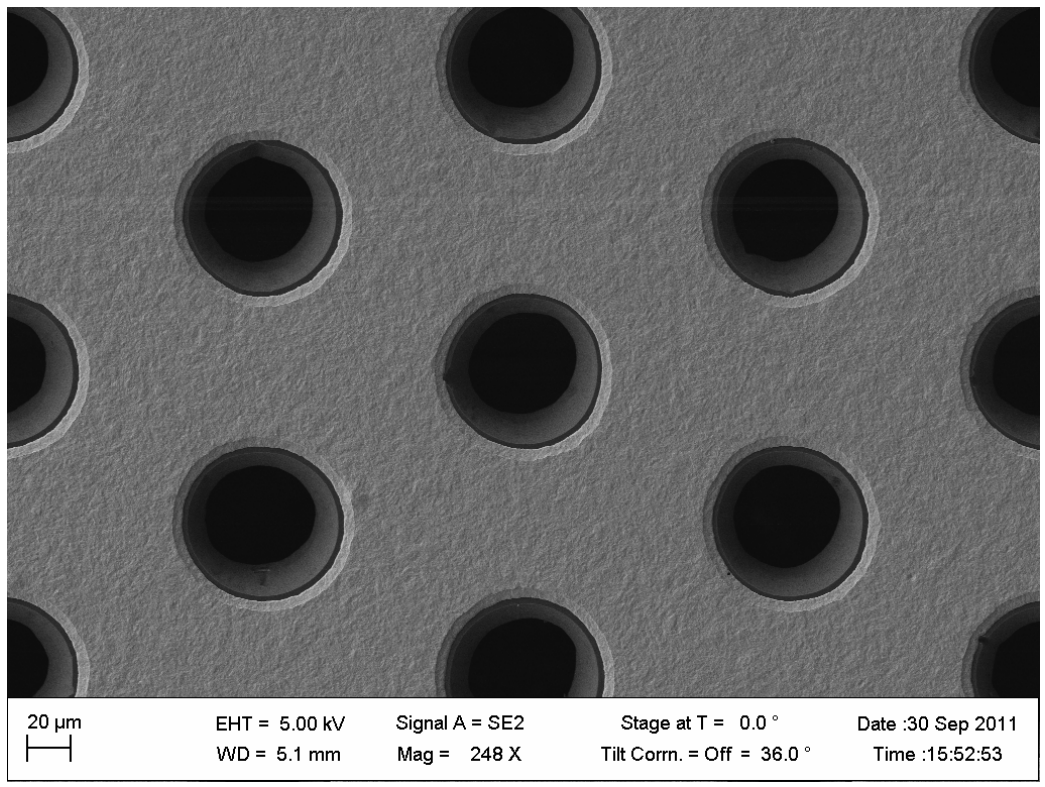
\includegraphics[width=.38\textwidth]{\imgpath/gem1.png}}}\hspace{1em}
\subfloat[][]{\adjustbox{valign=m}{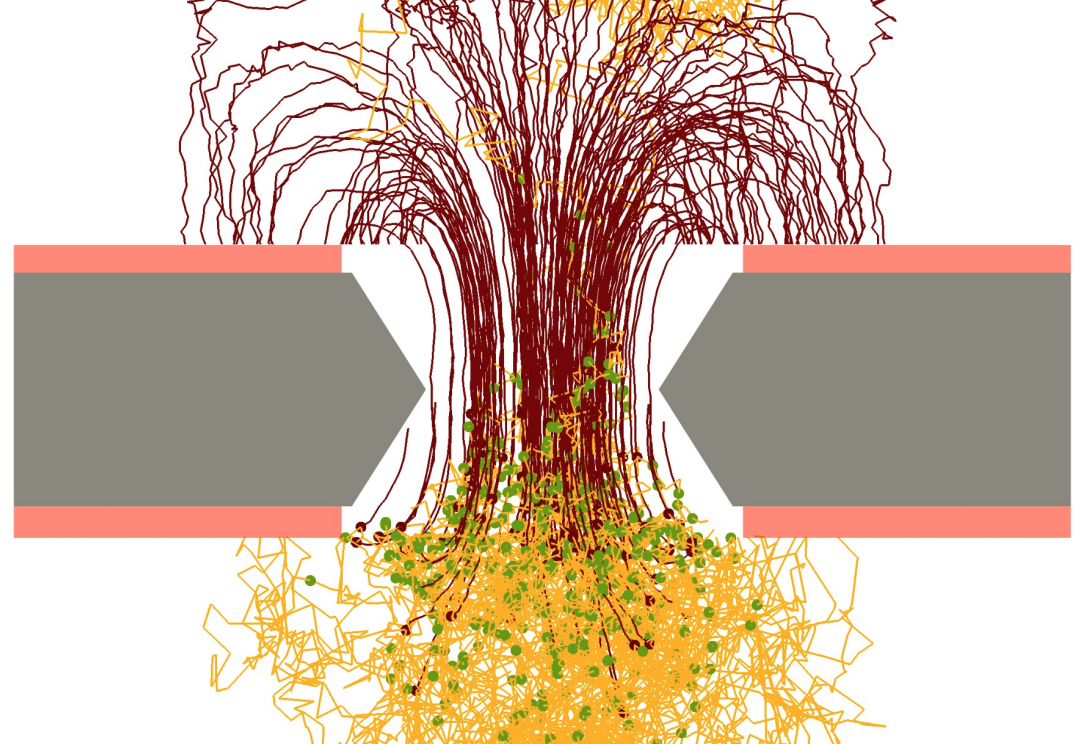
\includegraphics[width=.38\textwidth]{\imgpath/gem2c.png}}}\\
\subfloat[][]{\adjustbox{valign=m}{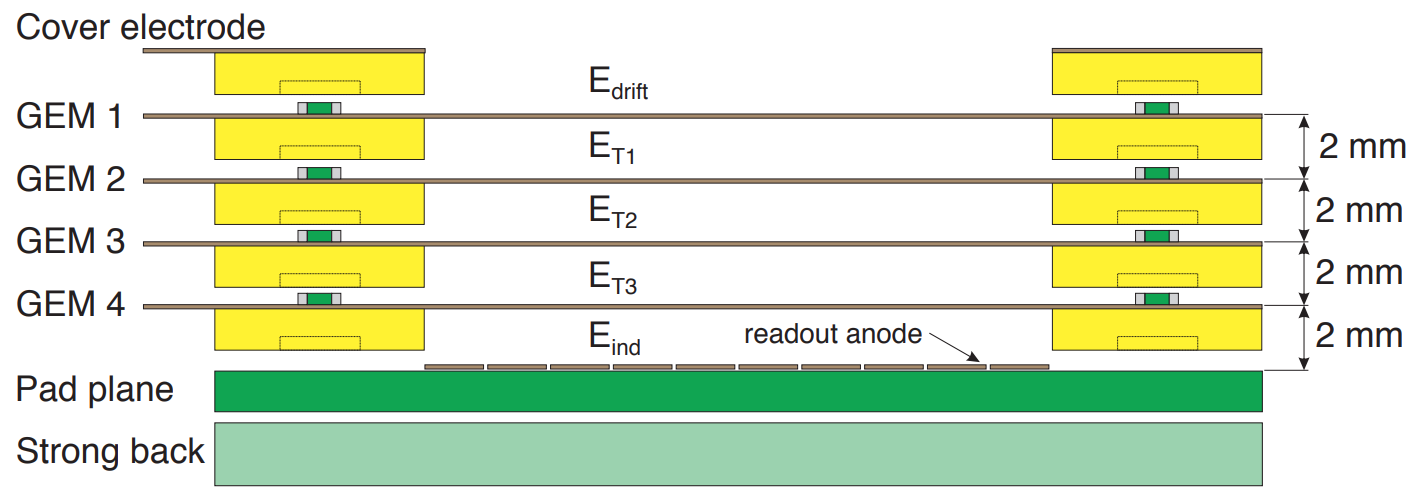
\includegraphics[width=.583\textwidth]{\imgpath/gem3.png}}}
\caption{\textbf{(a)} Electron microscope photograph of a GEM foil with hole pitch 140~$\mu$m. \cite{kalweitProductionLightFlavor2012} \textbf{(b)} Simulation of the charges in GEM holes. Dark lines represent ions and light lines electrons. Green dots mark multiplication site. \textbf{(c)} Schematic of the GEM setup at the upgraded ALICE TPC. \cite{peskovTechnicalDesignReport2014}}
\label{fig:alice:gems}
\end{figure}

\section{Inner Tracking Systems}

The Inner Tracking System \cite{collaborationALICEExperimentCERN2008, alicecollaborationAlignmentALICEInner2010} is a set of semiconductor-based detectors also located in the central barrel, but much closer to the beam pipe. ALICE uses the ITS for its great spatial resolution, which complements the TPC tracking and allows for precise determination of the primary vertex (PV) as well as secondary vertices of short-lived particle decays. Moreover, thanks to its fast processing, it is also used for triggering. The ITS consists of three detectors, each of two layers, which use different silicon detector technologies:
\begin{itemize}
\item Silicon Pixel Detector (SPD): uses an extremely granular pixel matrix closest to the IP, where particle densities are the highest.
\item Silicon Drift Detector (SDD): uses a similar technology based on drift cells. It is slightly less granular than the SPD but allows measuring of the deposited charge and thus PID based on $\mathrm{d}E/\mathrm{d}x$.
\item Silicon Strip Detector (SSD): uses a silicon detector with two arrays of strips, misaligned with $\Delta\phi \approx 2 \deg$, forming a lattice, on which a spatial coordinate can be determined. Similarly to the SDD, $\mathrm{d}E/\mathrm{d}x$ can also be measured.
\end{itemize}
Important parameters of the ITS sub-system can be found in Tab.~\ref{tab:alice:its} and the operating principles of the different silicon-based detector technologies used is discussed e.g.\ in Ref.~\cite{krammerSiliconDetectorsHigh2015, masciocchiLectureNotesSemiconductor2017}.

\begin{table}[h!]
\centering
\caption{Selection of parameters of the Inner Tracking System. \cite{collaborationALICEExperimentCERN2008}}
\label{tab:alice:its}
\begin{tabular}{|cc|ccc|}
\hline
\multicolumn{2}{|r|}{\parbox[b][1.2em]{2em}{} Detector} & SPD & SDD & SSD \\ \hline
\multicolumn{5}{l}{\parbox[b][1.2em]{1em}{} Parameter} \\
\hline
\multicolumn{2}{|l|}{\parbox[b][1.1em]{1em}{}Area (m$^2$)} & $0.07$ and $0.14$ & $0.42$ and $0.89$ & $2.09$ and $2.68$\\ \hline
\multicolumn{2}{|l|}{\parbox[b][1.1em]{1em}{}Cell size ($\mu$m)} & $50\times 425$ & $150\times 300$ & $95\times 40000$\\ \hline
\multicolumn{2}{|l|}{\parbox[b][1.1em]{1em}{}Number of cells (M)} & $9.84$ & $23$ & $2.6$\\ \hline
\multicolumn{2}{|l|}{\parbox[b][1.1em]{1em}{}Spatial resolution ($\mu$m)} & $12$ in $r\phi$, $100$ in $z$ & $38$ in $r\phi$, $28$ in $z$ & $20$ in $r\phi$, $830$ in $z$\\ \hline
\multicolumn{2}{|l|}{\parbox[b][1.1em]{1em}{}Mat.\ budget, layers $X/X_0$} & $1.14\%$ and $1.14\%$ & $1.13\%$ and $1.26\%$ & $0.83\%$ and $0.86\%$\\ \hline
\multicolumn{2}{|l|}{\parbox[b][1.1em]{1em}{}Mat.\ budget, supp.\ $X/X_0$} & $0.52\%$ & $0.25\%$ & $0.53\%$\\ \hline
\end{tabular}
\end{table}

\begin{figure}[!h]
\subfloat[][]{\adjustbox{valign=m}{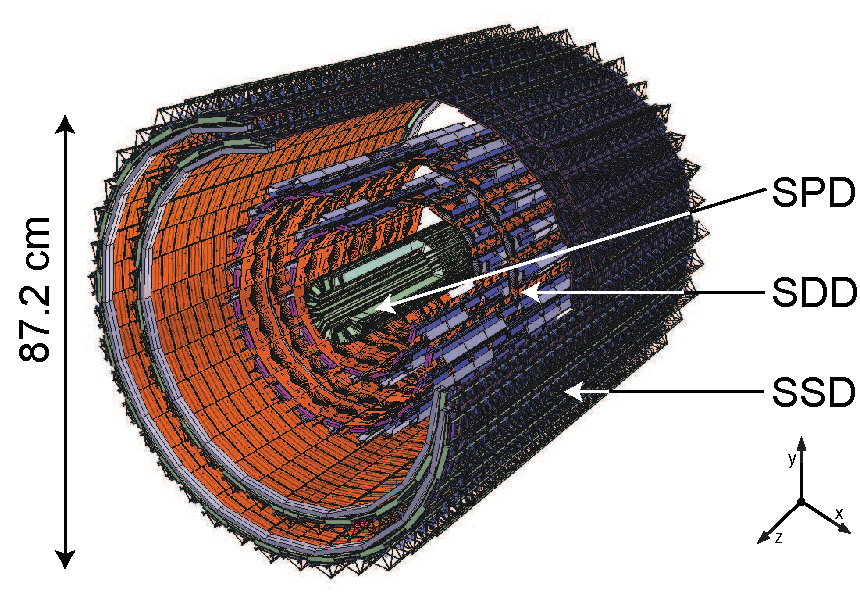
\includegraphics[width=.45\textwidth]{\imgpath/its.pdf}}}%\hspace{1em}
\subfloat[][]{\adjustbox{valign=m}{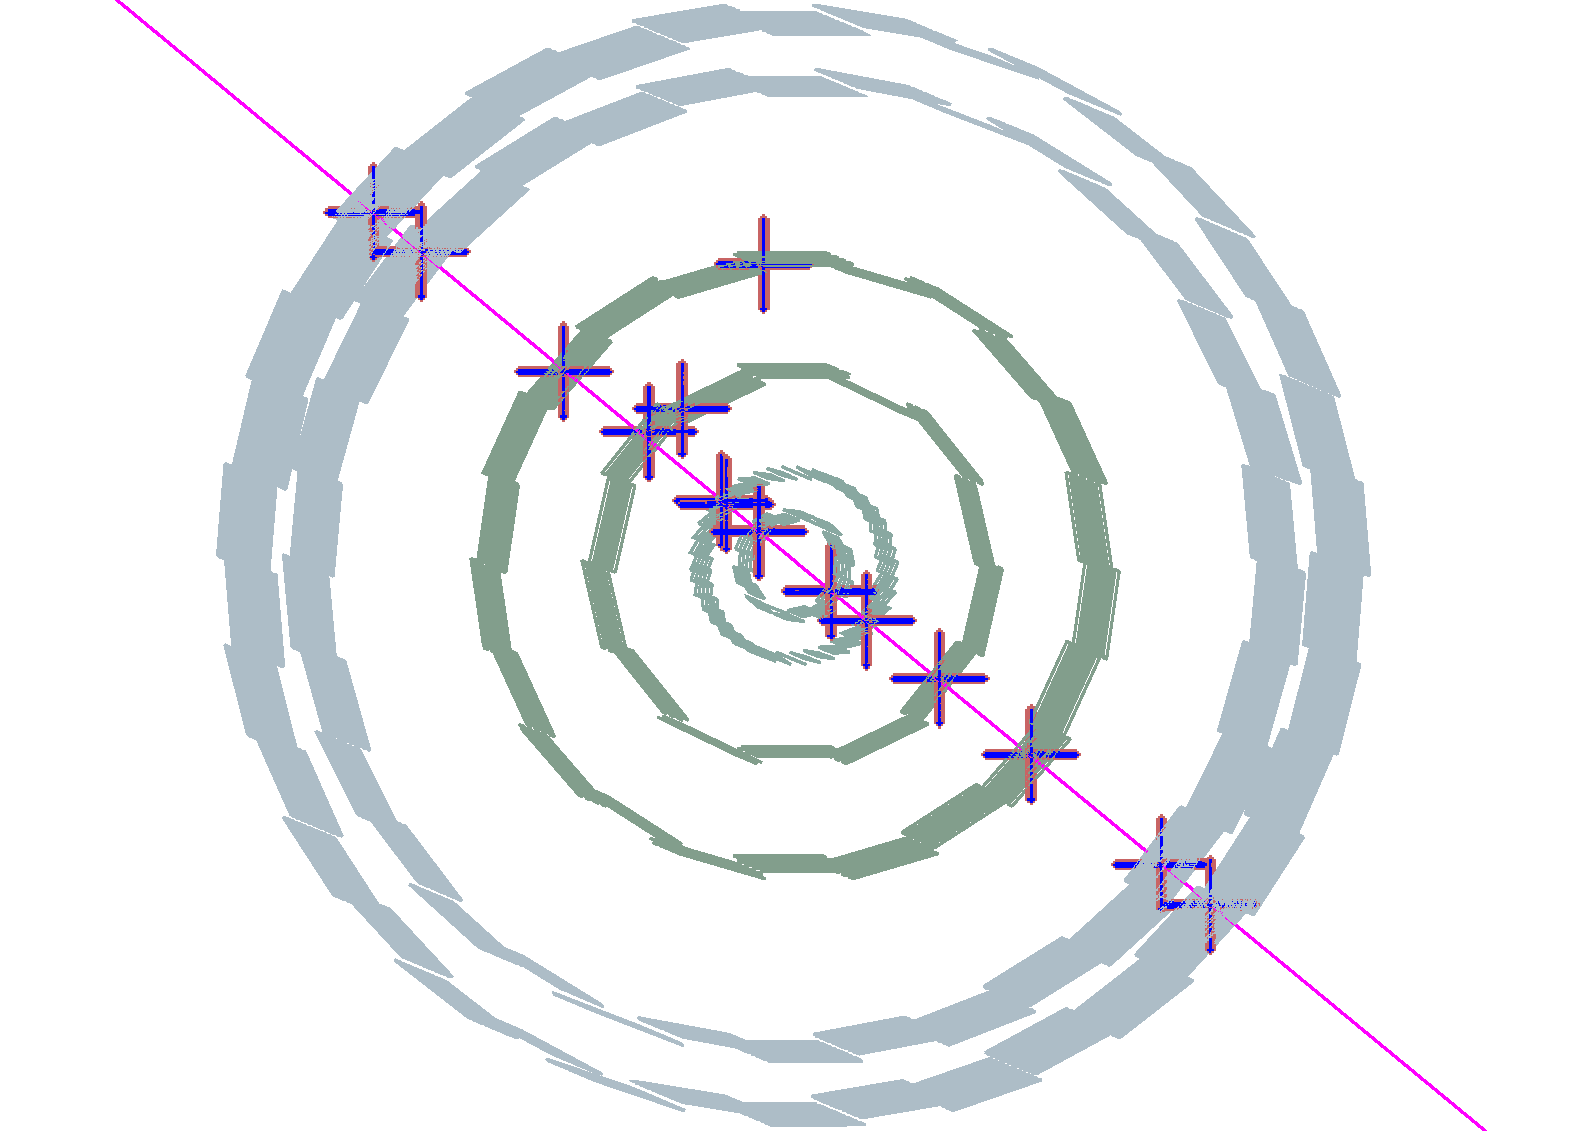
\includegraphics[width=.45\textwidth]{\imgpath/itscosmic.pdf}}}
\caption{\textbf{(a)} Three-dimensional model of the ITS sub-system in ALICE detector simulations. \textbf{(b)} Display of a cosmic event detected by the ITS. \cite{alicecollaborationAlignmentALICEInner2010}}
\label{fig:alice:its}
\end{figure}

\section{\VOA and \VOC}

The \VOA and \VOC\footnote{In ALICE, the ``A-side" points in the counter-clockwise and the ``C-side" in the clockwise direction of the LHC beam pipe, aligned with the $z$-axis. The C-side contains the muon system.} are two arrays of plastic scintillator counters, with PMT read-outs, together forming the V$0$ sub-system \cite{alicecollaborationPerformanceALICEVZERO2013}. They are placed asymmetrically on the $z$-axis with respect to the IP in order to accomodate the hadron absorber used in the muon tracking system of ALICE. Their inner and outer radii are $4.3$ and $42.2$~cm for the \VOA and $4.5$ and $32$~cm for the \VOC. Furthermore, they are segmented into 8 sectors azimuthally and 4 sectors radially. This is usually not granular enough for tracking, but sufficient for forward multiplicity estimation (combining amplitudes of both parts, referred to as \VOM) or determination of the event plane. 

Thanks to its speed, the V$0$ is also used for triggering. Additionally, since they can be used in coincidence, interactions of the protons/nuclei with residual gas in the beam pipe outside of the IP can be identified based on the different time information and rejected. The two detectors are visualised in Fig.~\ref{fig:alice:vzero}.

\begin{figure}[!h]
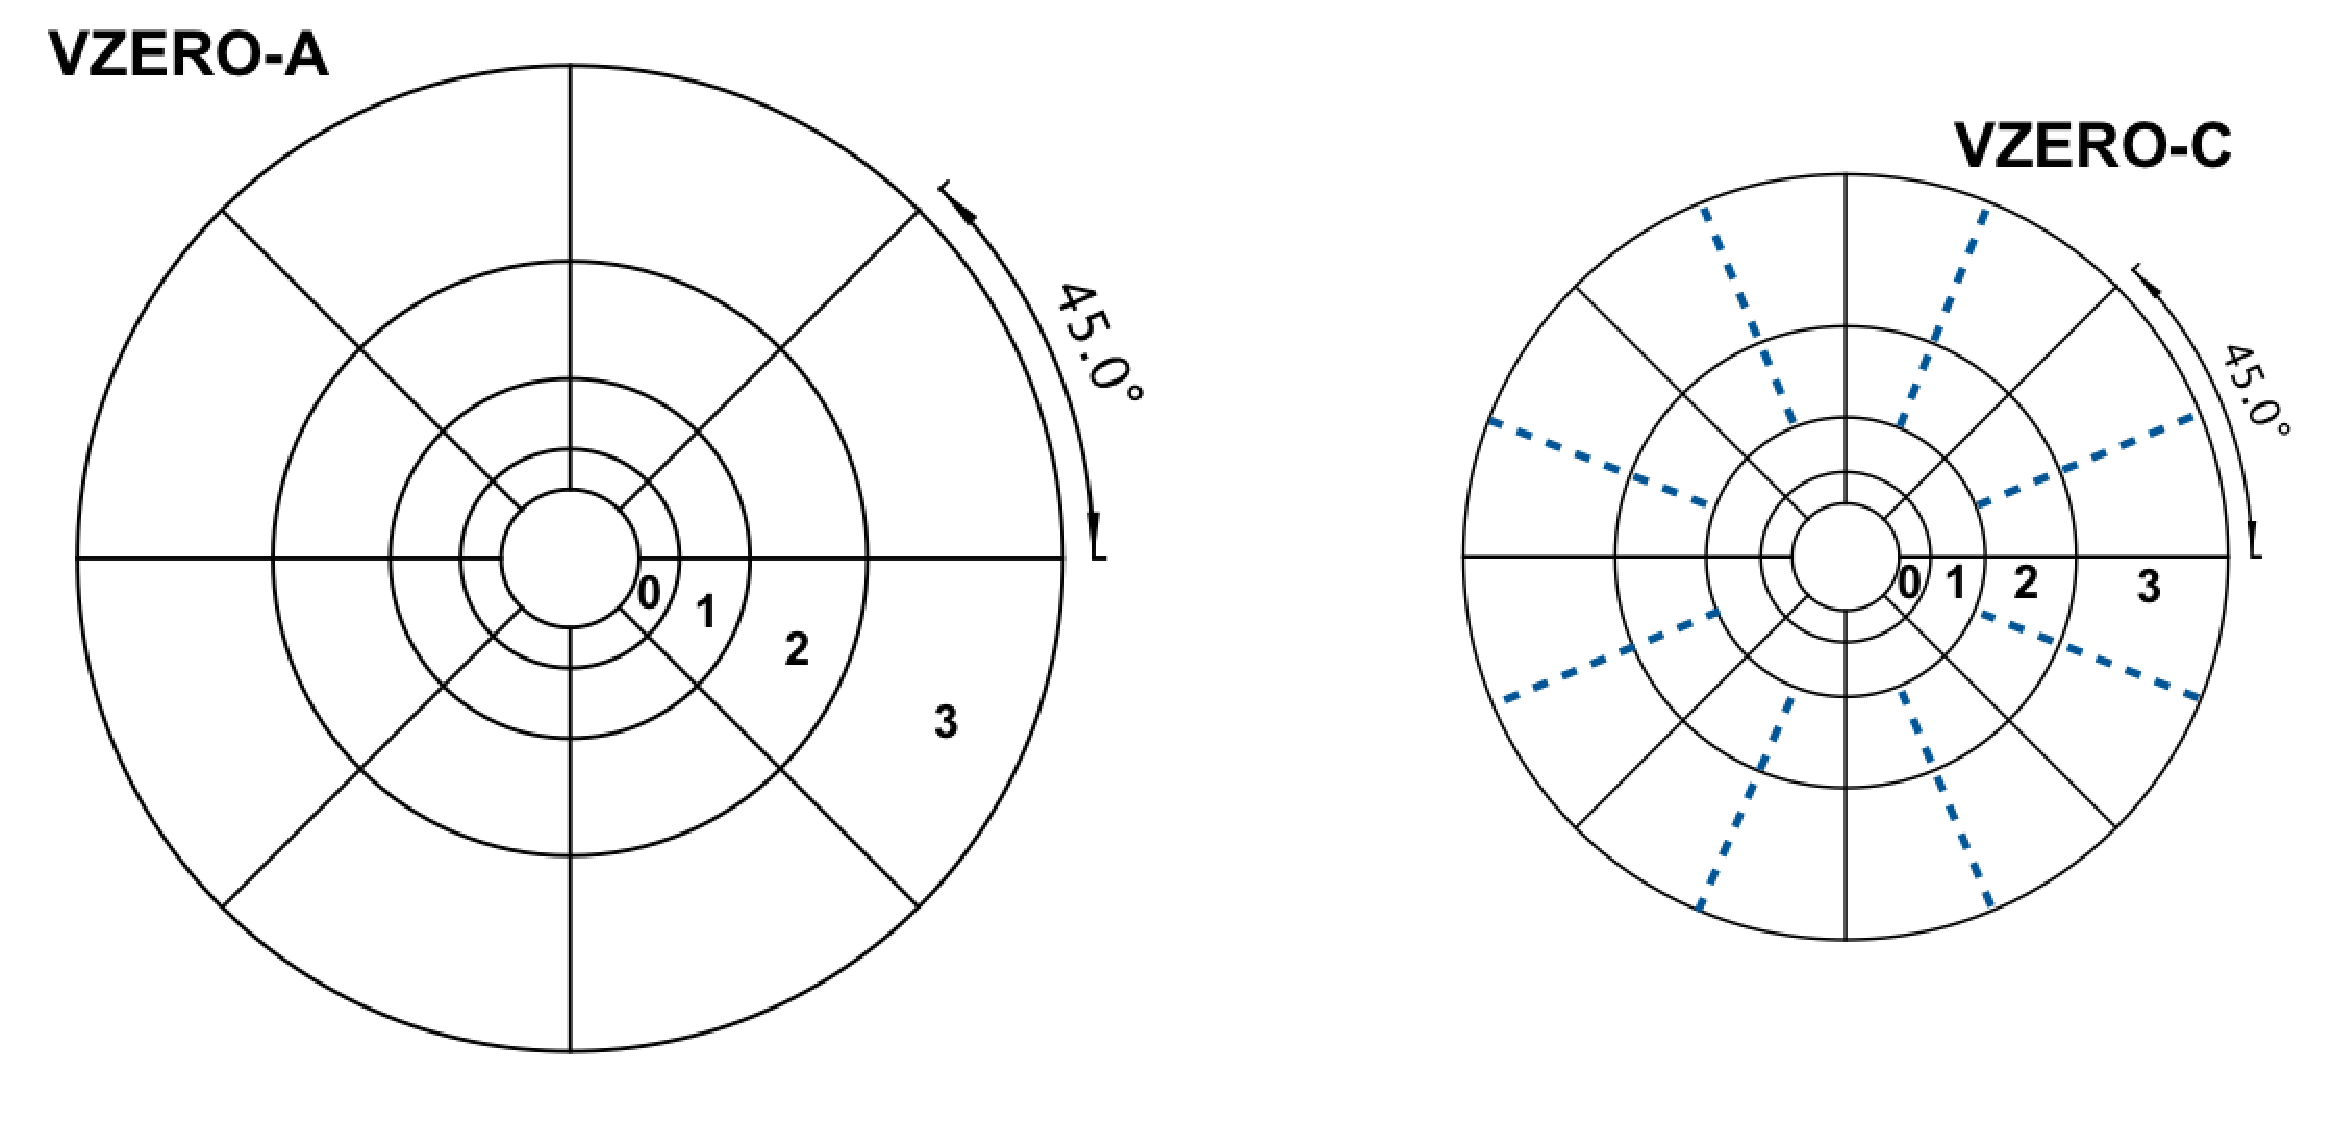
\includegraphics[width=.65\textwidth]{\imgpath/vzero.eps}\caption{Schematic of the \VOA and \VOC scintillator arrays. \cite{alicecollaborationPerformanceALICEVZERO2013}}
\label{fig:alice:vzero}
\end{figure}
